\subsection{Untersuchung einzelner Streuwinkel}

Zur Kalibrierung des organischen Szintillators wurde die WCKM verwendet. Dafür wurden immer koinzidente Ereignisse aufgenommen und die gemessenen Detektorkanäle in einem zweidimensionalen Histogramm gegeneinander aufgetragen. Vor der eigentlichen Kalibrierung wurden jedoch einzelne Streuwinkel untersucht. Dafür wurde die $^{22}$Na-Probe mithilfe des Roboterarms an verschiedene Koordinaten gefahren (s. Tabelle \ref{kali_szint_coords}). Die entsprechenden Histogramme sind in Abbildung \ref{kali_szint_winkelabh} zu sehen.

\begin{table}[h]
    \centering
    \begin{tabular}{|c | c |c |}
        \hline
        Koordinaten $(x,y,z)$  & Streuwinkel & Messzeit \\
        \hline
        $(-33, 10, 7)$ & \SI{70.7}{\degree} & \SI{60}{\minute} \\
        $(-33, 4, 15)$ & \SI{60.0}{\degree} & \SI{30}{\minute} \\
        $(-33, 6, 20)$ & \SI{50.2}{\degree} & \SI{30}{\minute} \\
        $(-33, 9, 24)$ & \SI{41.2}{\degree} & \SI{30}{\minute} \\
        $(-33, 20, 27)$ & \SI{20.3}{\degree} & \SI{30}{\minute} \\
        \hline
    \end{tabular}
    \caption{Angefahrene Koordinaten der $^{22}$Na-Probe, daraus resultierender Streuwinkel (grob) und Messzeit an dem jeweiligen Punkt. Die Winkel wurden bestimmt durch die Formel $\phi = \arctan{\frac{\triangle z}{\triangle y}}$, wobei $\triangle$ immer die Differenz zur Koordinate des Detektors ist. Diese haben wir mit $(x,y,z) = (-33, 30, 0)$ abgeschätzt.}
    \label{kali_szint_coords}
\end{table}

\begin{figure}[ht]
	\centering
    \begin{tabular}{c c}
        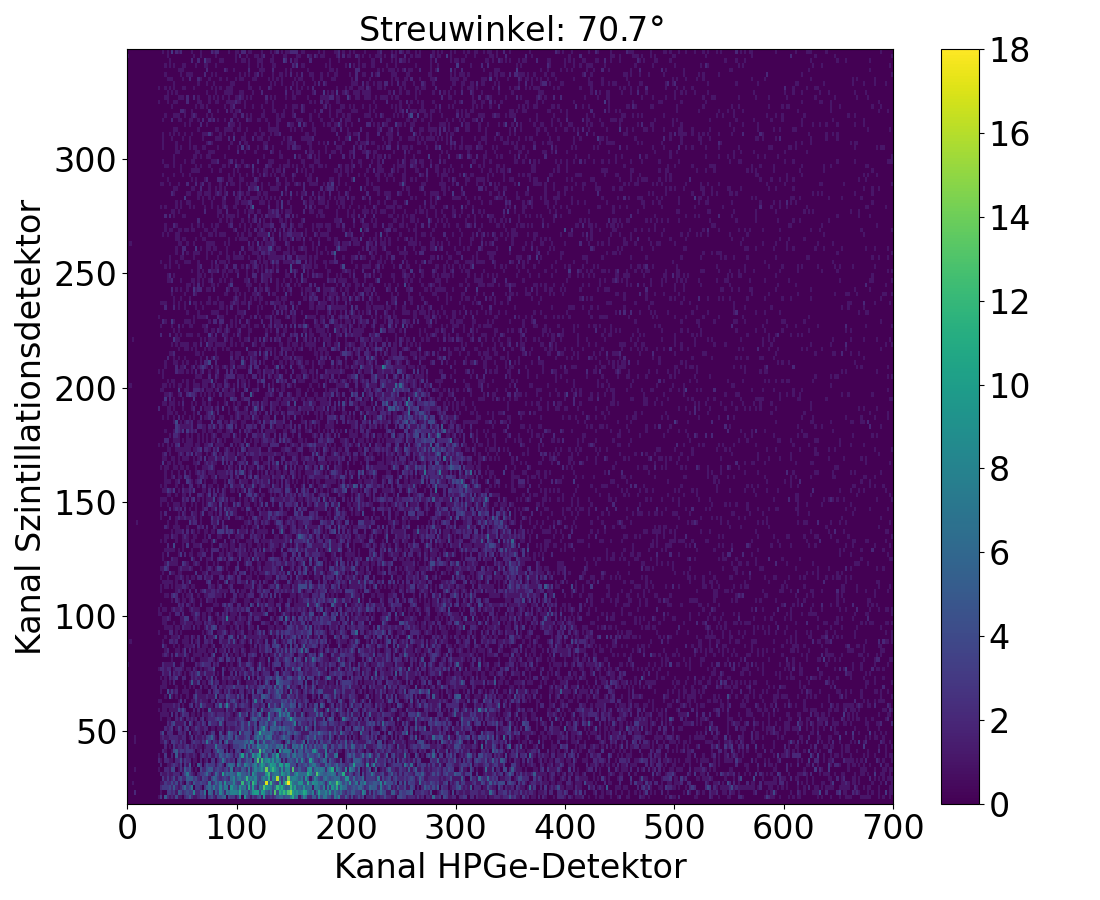
\includegraphics[width=0.49\textwidth]{images/kali_szint_Streuwinkel_70_v2.png} & 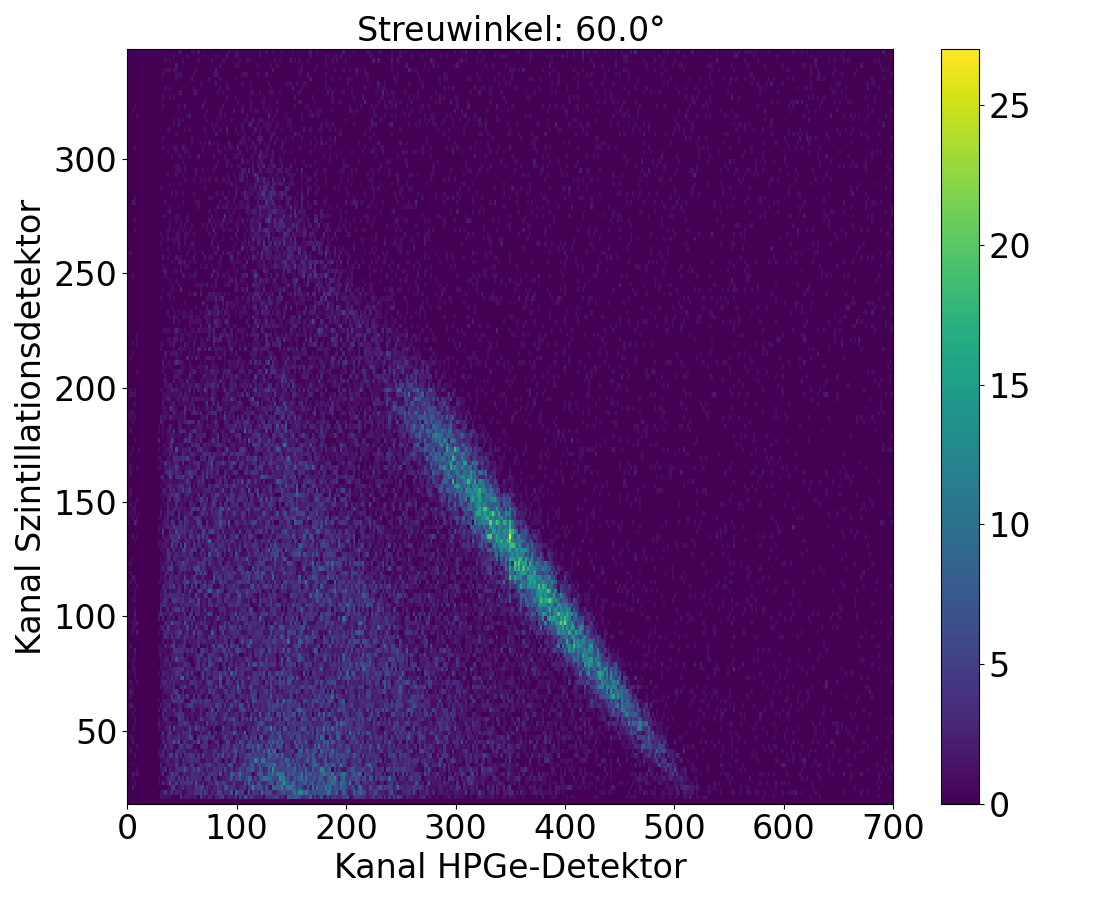
\includegraphics[width=0.49\textwidth]{images/kali_szint_Streuwinkel_60_v2.png} \\ 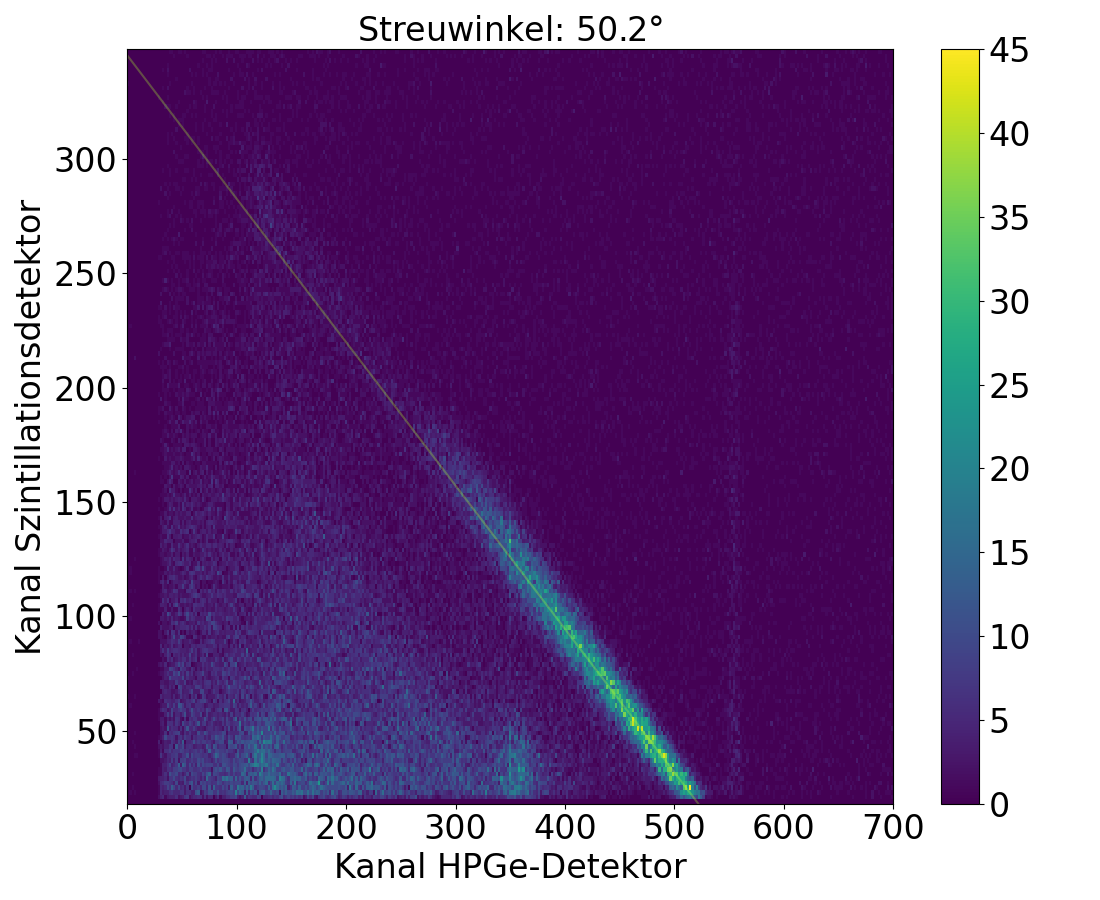
\includegraphics[width=0.49\textwidth]{images/kali_szint_Streuwinkel_50_v2.png} & 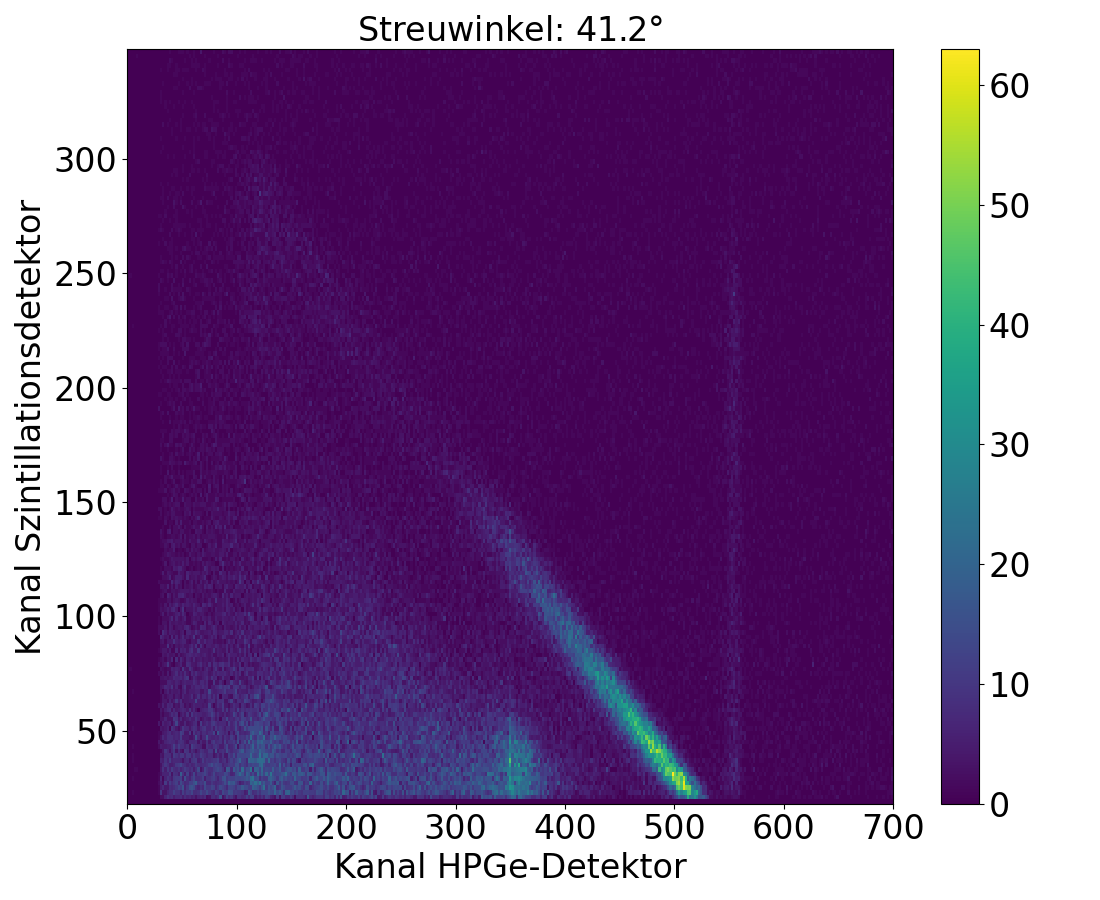
\includegraphics[width=0.49\textwidth]{images/kali_szint_Streuwinkel_40_v2.png} \\\
        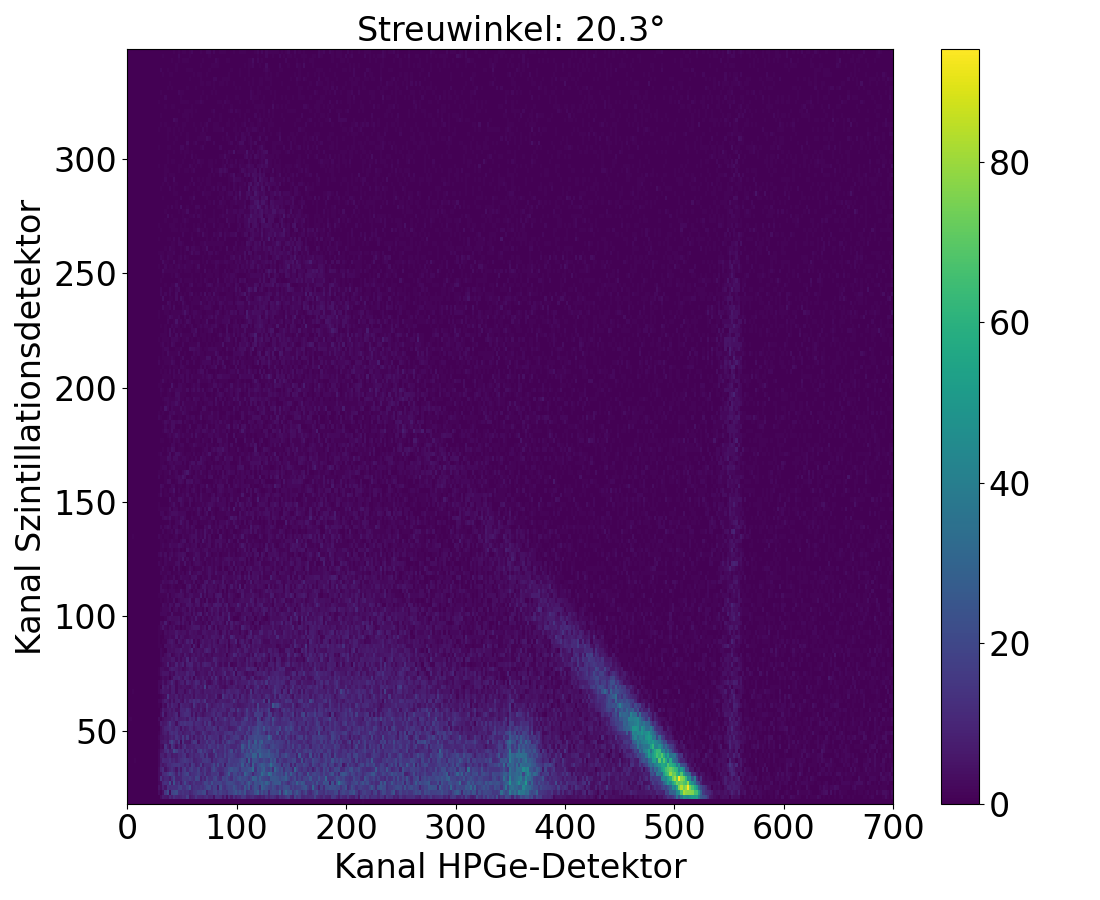
\includegraphics[width=0.49\textwidth]{images/kali_szint_Streuwinkel_20_v2.png} & \\
    \end{tabular}
	\caption{Histogramme der koinzidenten Ereignisse für verschiedene Streuwinkel im Szintillator bei Nutzung einer $^{22}$Na-Probe, für den Streuwinkel von \SI{50.2}{\degree} ist die gesuchte lineare Beziehung der Detektorkanäle bei koinzidenten Ereignissen eingetragen}
	\label{kali_szint_winkelabh}
\end{figure}

Man erkennt in diesen Histogrammen einige Dinge. Zum ersten verschiebt sich mit sinkendem Streuwinkel der Bereich, in dem besonders viele Ereignisse auftreten, zu höheren Kanälen im HPGe-Detektor und zu niedrigeren im Szintillationsdetektor. Auch sieht man sofort den linearen Zusammenhang der gemessenen Kanäle (Energien). Diesen kann man beobachten für jede von der Strahlungsquelle abgegebene Energie der Photonen, jedoch ist die im Bild rechte Gerade deutlich schwerer zu erkennen. Man kann daraus folgern, dass, wie bereits diskutiert, bei koinzidenten Ereignissen häufig die Energie, die bei einer Compton-Streuung nicht im Szintillator deponiert wird, im HPGe-Detektor deponiert wird. Man kann anhand der Intensitäten der Punkte auf der Geraden (siehe Farbskala) außerdem darauf schließen, dass ein Streuen in kleineren Winkeln wahrscheinlicher ist und damit in der selben Messzeit öfter auftritt. Man muss dazu erwähnen, dass für den Streuwinkel von \SI{70.7}{\degree} eine Bleiverschirmung zwischen Quelle und Szintillator stand, womit dieses Histogramm für diese Aussage nicht herangezogen werden kann.

\subsection{Energiekalibrierung des organischen Szintilators}

Für die Kalibrierung wurden die diagonalen, linearen Bereiche gefittet und dann der Schnittpunkt der Geraden mit der y-Achse gesucht. Dies entspräche dann nämlich dem Fall, dass die im HPGe-Detektor deponierte Energie $0$ ist und sämtliche Energie des Photons im Szintillator deponiert wurde. Ein Beispiel für einen Fit ist in Abb. \ref{kali_szint_bsp_fit} zu sehen.

\begin{figure}[ht]
	\centering
    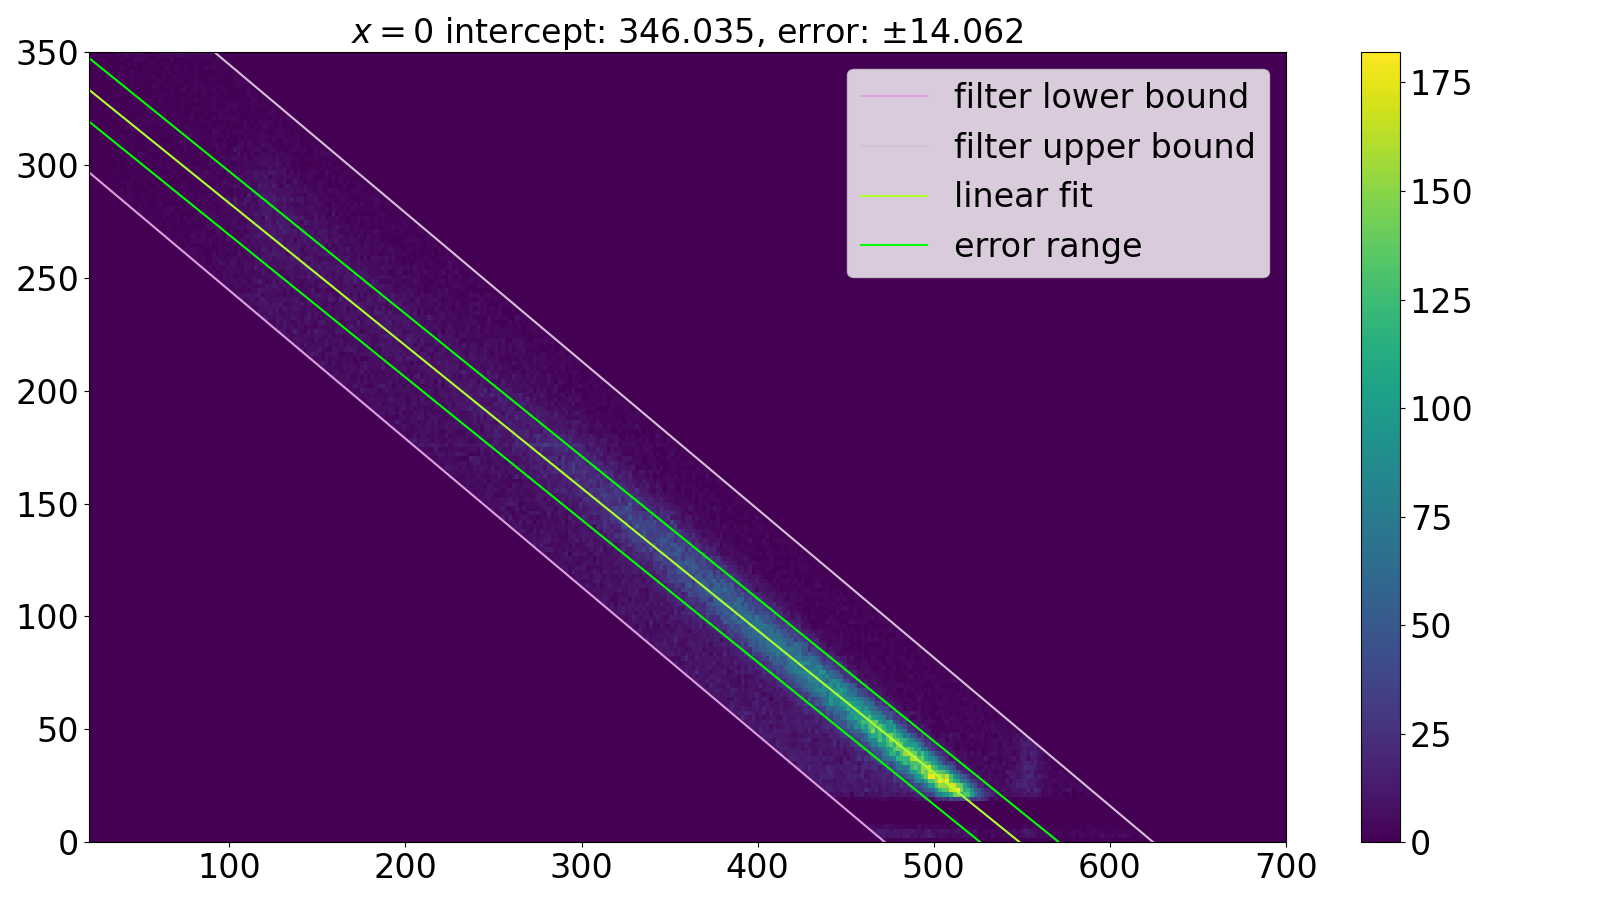
\includegraphics[width=0.98\textwidth]{images/kali_szint_fit_Na22.png}
	\caption{Beispiel für die verwendete Prozedur der linearen Regression für Nutzung einer $^{22}$Na-Probe. Zuerst wurde der grobe Bereich des linearen Zusammenhangs ausgeschnitten. Danach wurde eine lineare Regression der Daten durchgeführt. Zuletzt wurden zwei Geraden äquidistant und parallel zur Regressionsgeraden verschoben bis $ 68 \% $ ($1 \sigma$) aller Punkte des ausgeschnittenen Bereichs innerhalb dieser Geraden liegen. Die Schnittpunkte dieser Geraden mit der y-Achse stellen unsere Messunsicherheit dar.}
	\label{kali_szint_bsp_fit}
\end{figure}

Bei der Kalibrierung mit $^{22}$Na wurden die Daten der Streuwinkelmessung und eine zweistündige Messung, bei der die Probe in einem Kreisbogen gefahren wurde, benutzt. Bei der Kalibrierung mit $^{133}$Ba wurde die Probe \SI{4.5}{\hour} im Kreisbogen um den Szintillator gefahren. Die Ergebnisse des Fittings sind in Tabelle \ref{kali_szint_Energien} zu sehen.

\begin{table}[h]
    \centering
    \begin{tabular}{|c | c | c | c|}
        \hline
        Element & Photonenenergie & Kanal & Unsicherheit im Kanal \\
        \hline
        $^{22}$Na & \SI{511.00}{\kilo\electronvolt} & 346 & 14 \\
        $^{22}$Na & \SI{1274.54}{\kilo\electronvolt} & 906 & 15 \\
        $^{133}$Ba & \SI{356.02}{\kilo\electronvolt} & 229 & 9 \\
        \hline
    \end{tabular}
    \caption{Zerfallsenergien und zugeordnete Kanäle im Szintillationsdetektor. Leider ist nur eine der Linien der $^{133}$Ba-Quelle in den Daten gut zu erkennen.}
    \label{kali_szint_Energien}
\end{table}

Auch hier wird wieder ein linearer Zusammenhang zwischen Kanälen und Energien angenommen. Dieser Fit wurde ebenfalls mithilfe des in \cite{Fit_bivariate} beschriebenen Algorithmus nach York durchgeführt, wobei für die Fehler in der Energie wieder extrem kleine Werte angenommen wurden.
Damit ergibt sich die Kalibrierung für den Szintillator:
\begin{gather}
    E_{\text{Szintillator}} (K) = [(1.357 \pm 0.035) \cdot K + (44.199 \pm 16.521)] \ \si{\kilo\electronvolt}
\end{gather}
Wobei natürlich $K$ der Kanal des ADC ist.
Der relative Fehler des Anstiegs ist also etwa \SI{3}{\percent}.
Dieser ist damit sehr ähnlich zu dem des HPGe-Detektors.
Das ist gut, denn wir nehmen effektiv eine Kalibrierung unter Ausnutzung der Genauigkeit des HPGe-Detektor vor.
Der Fehler des Schnittpunktes mit der y-Achse ist wie schon beim HPGe-Detektor schwerer einzuschätzen.
Es handelt sich dabei letztlich um den Hauptanteil der Unsicherheit der Energieauflösung.
